\documentclass{article}
\usepackage{graphicx} % Required for inserting images
\usepackage{float} % For [H] float placement
\usepackage{booktabs}
\usepackage{caption}
\usepackage{adjustbox}
\usepackage[utf8]{inputenc}  % This is for old compilers, but good practice
\usepackage[T1]{fontenc}    % This is for correct character encoding (accents, ñ, etc.)
\usepackage[spanish,es-tabla]{babel}
\usepackage[margin=3cm]{geometry} % This line changes the margins
\usepackage{subcaption}
\usepackage{url}
%for citations
\usepackage[style=apa, backend=biber]{biblatex}
\usepackage{hyperref}
\addbibresource{references.bib}

%for notes and corrections
\usepackage{soul}
\usepackage{xcolor}
\usepackage{comment}
%para tablas largas
\usepackage{longtable}


\title{Cuando OXXO llega a la cuadra: El efecto de OXXO en XXXXX (ni idea por ahora)}
\author{Sophia Aristizábal Flórez}

\begin{document}

\maketitle

\section{Introduction}
Desde su llegada en 2009, OXXO se ha consolidado como una de las principales cadenas de conveniencia en Colombia \parencite{m_2025}. Su modelo basado en la accesibilidad de productos básicos plantea la incógnita de si estas tiendas desencadenan la desaparición de minoristas informales. \\

\hl{En dicho contexto, esta investigación buscará responder si la presencia de OXXO causa una disminución en la actividad informal en su entorno cercano en Bogotá.} La respuesta a esta pregunta ayuda a comprender posibles cambios en las dinámicas económicas locales: ¿estamos frente a un fenómeno de desplazamiento de formas tradicionales de autoempleo o a un proceso de formalización y competencia renovada en contextos urbanos en desarrollo? \\

Algunos estudios sugieren que los minoristas informales no desaparecen sino que se adaptan y compiten \parencite{marcos2022}. Otros, por otro lado, no encuentran efectos significativos sobre el empleo informal a nivel municipal \parencite{delgado2024}. \hl{HIPÓTESIS}\\

La investigación usará datos de las secretarías de planeación y de movilidad de Bogotá y dividirá la ciudad en Zonas de Análisis de Transporte  (ZAT).  Utilizando el método de two-way fixed effects (TWFE), se evaluará la llegada escalonada de los OXXO en las zonas y \hl{su efecto en la proporción de trabajadores independentes que llegan a trabajar a dicho ZAT, utilizada como proxy indirecto de la actividad económica informal local.} 

\begin{comment}
⚠️ Limitaciones
Heterogeneidad del grupo
No todos los independientes son informales: hay abogados, consultores, profesionales freelance que nada tienen que ver con comercio de barrio.
Eso introduce “ruido” en la medición.
Movilidad laboral
Si un tendero deja de ser independiente, no necesariamente aparece como desempleado: puede formalizarse, migrar a otro sector o trabajar en otro barrio. Eso diluye el efecto.
Datos de movilidad ≠ actividad comercial directa
La EOD captura desplazamientos, no unidades de negocio. Entonces el proxy es indirecto.

El 80\% de los trabajadores independientes son informales, siendo la mayoría trabajadores por cuenta propia.
https://www.bbvaresearch.com/publicaciones/colombia-empleo-no-asalariado-gran-jalonador-del-empleo-nacional/

https://www.larepublica.co/globoeconomia/colombia-es-el-pais-de-la-ocde-que-con-mayor-numero-de-trabajadores-independientes-3215200

https://www.dane.gov.co/files/operaciones/EMICRON/bol-EMICRON-PanaderiasTiendasBarrio-2023.pdf

\end{comment}

\newpage

\section{Revisión de literatura}

La expansión de grandes cadenas minoristas ha suscitado de forma recurrente la pregunta sobre sus efectos en el mercado laboral. Algunos estudios, por ejemplo, han exáminado  cómo las grandes tiendas de descuento inciden en las dinámicas laborales locales de economías desarrolladas. \\

Una de estas investigaciones explora cómo la entrada de Walmart en nuevos condados de Estados Unidos reduce, a mediano y largo plazo, el empleo y las ganancias de tiendas minoristas medianas y pequeñas \parencite{basker2005}. En contraste, \textcite{cho2015} encuentran para Corea que la llegada de estas grandes cadenas impulsa el empleo minorista local. Estas marcadas diferencias sugieren que el efecto depende del nivel de desarrollo y madurez del sector minorista en cada economía. \\

Por tanto, el debate ha cobrado relevancia en economías en desarrollo, donde predominan la informalidad, los negocios infomales minoristas (como las tiendas de barrio) y la coexistencia con supermercados tradicionales. \\

\textcite{marcos2022} exploró directamente cómo las cadenas de conveniencia (como OXXO) afectaban a las tiendas de barrio en México. Su estudio plantea que estas cadenas actúan como sustitutos de los pequeños negocios, al presentar una traslape significativo en sus ofertas de productos. Para abordar la no aleatoriedad en la entrada temporal y espacial de estas cadenas, empleó una variable instrumental y encontró que su llegada reducía en un 15\% el número de tiendas de barrio en la zona. Este efecto se explica principalmente por la menor creación de nuevos establecimientos, más que por el cierre masivo de los ya existentes. \\

En Colombia, la literatura se ha concentrado en el efecto de tiendas de descuento duro (D1, ARA y Justo y Bueno) a nivel municipal sobre diferentes indicadores del mercado laboral. \textcite{delgado2024} muestran que su llegada aumenta el empleo formal en 1.7 pp. Y aunque estas también reducen los ingresos de los minoristas informales, no encontraron efectos significativos sobre el empleo informal. Sin embargo, este análisis excluyó tanto a las cadenas de conveniencia (incluyendo OXXO) como a las ciudades capitales, al presumir que en ellas el impacto de estas tiendas en el mercado laboral sería marginal. \\

Como se evidencia en la literatura, pocos estudios analizan los efectos de grandes cadenas minoristas a nivel intraurbano, diferenciando entre barrios o zonas. \hl{Esta investigación busca llenar ese vacío al examinar el impacto de OXXO sobre la actividad económica informal en Bogotá}. Esta ciudad concentra cerca del 40–50\% de sus sucursales \parencite{godoy2025}, lo que la convierte en un escenario privilegiado para observar sus efectos en la dinámica laboral y comercial local. Dicho enfoque permite explorar la heterogeneidad espacial del fenómeno (según zonas y características socioeconómicas) y abrir un nuevo debate sobre la relación entre cadenas modernas, tiendas tradicionales e informalidad laboral, en un contexto donde la formalización del empleo es una prioridad.\\

\section{Estadísticas Descriptivas} 

\subsection{Descripción de los datos}
Los resultados de esta investigación emplean cinco fuentes de datos. A partir del RUES \footnote{\url{https://www.rues.org.co}} y de GoogleMaps API se identificaron el año de apertura, cierre y localización de cada sucursal de OXXO, D1, Justo\&Bueno y ARA, estas últimas incluidas por su posible influencia en la localización de los OXXO. Con la Encuesta de Calidad de Vida de Bogotá 2007 \footnote{\url{https://www.dane.gov.co/index.php/estadisticas-por-tema/salud/calidad-de-vida-ecv/encuesta-nacional-de-calidad-de-vida-2007-bogota}} se construyeron los controles de línea base, mientras que con Mapas-Bogotá se obtuvo los controles fijos \footnote{\url{https://mapas.bogota.gov.co}}. Finalmente, las Encuestas de Movilidad (2011, 2015, 2019 y 2023) \footnote{\url{https://www.simur.gov.co/encuestas-de-movilidad}} permitieron construir la variable dependiente. Esta mide por año la proporción de trabajadores independientes que se movilizan a trabajar al ZAT i sobre el total de los trabajadores que se movilizan a dicho ZAT:\\

\begin{equation}
    proporcion\_independientes_{i,t}=\frac{trabajadores\_independientes_{i,t}}{total\_trabajadores_{i,t}} ; \quad \forall i, t
\end{equation}


A continuación, se describe las variables utilizadas:

\begin{longtable}{p{0.25\linewidth} p{0.45\linewidth} p{0.25\linewidth}}
\caption{Descripción de variables y fuentes de datos}
\label{tab:variables_descripcion}
\\
\toprule
\textbf{Variable} & \textbf{Descripción} & \textbf{Fuente de los datos} \\
\midrule
\endhead
\midrule
\multicolumn{3}{l}{\textbf{Variable dependiente}} \\
\midrule
proporción independientes & Proporción de independientes en el ZAT ese año & Encuestas de movilidad (2011, 2015, 2019, 2023) \\
\midrule
\multicolumn{3}{l}{\textbf{Variable de tratamiento escalonado}} \\
\midrule
Tiene OXXO ($=1$) & Si el ZAT tiene OXXO(s) ese año & RUES y Google Maps API \\
\midrule
\multicolumn{3}{l}{\textbf{Controles de línea base}} \\
\midrule
Densidad urbana por upz 2009 & Densidad urbana (can hab/ha) por UPZ en el 2009 & Secretraría Distrital de Planeación de Bogotá \\
\midrule
Área urbana por upz 2009 & Área en hectáreas de la UPZ clasificada como suelo urbano en el 2009 & Secretraría Distrital de Planeación de Bogotá \\
\midrule
Poblacion urbana por upz 2009 & Cantidad de habitantes que viven en suelo urbano por UPZ en el 2009 & Secretraría Distrital de Planeación de Bogotá \\
\midrule
Habitantes por localidad en 2007 & Número de habitantes por localidad en el 2007 & Encuesta de Calidad de Vida de Bogotá 2007 \\
\midrule
Cantidad de personas por hogar 2007 & Número promedio de personas en el hogar por localidad en el 2007 & Encuesta de Calidad de Vida de Bogotá 2007 \\
\midrule
Indice de condiciones de vida 2007 & Indice de condiciones de vida promedio por localidad en el 2007 & Encuesta de Calidad de Vida de Bogotá 2007 \\
\midrule
Gasto promedio mensual 2007 & Gasto promedio mensual en el hogar por localidad en el 2007 & Encuesta de Calidad de Vida de Bogotá 2007 \\
\midrule
\multicolumn{3}{l}{\textbf{Controles fijos en el tiempo}} \\
\midrule
Estrato promedio del ZAT & Estrato promedio del ZAT, que oscila de 1 a 6 & Mapas Bogotá - Infraestructura de Datos Espaciales de Bogotá (IDECA) \\
\midrule
Estaciones de transmilenio cercanas & Cantidad de estaciones de transmilenio dentro o cercanos al ZAT & Mapas Bogotá - Infraestructura de Datos Espaciales de Bogotá (IDECA) \\
\midrule
Cantidad acceso a vías arteriales & Cantidad de vías arteriales dentro o cercanos al ZAT & Mapas Bogotá - Infraestructura de Datos Espaciales de Bogotá (IDECA) \\
\midrule
\multicolumn{3}{l}{\textbf{Controles resagados de tiendas de cadena}} \\
\midrule
Tiene D1s (=1) & El ZAT tiene D1s el periodo anterior al año analizado & RUES y Google Maps API \\
\midrule
Tiene ARAs (=1) & El ZAT tiene ARAs el periodo anterior al año analizado & RUES y Google Maps API \\
\midrule
\multicolumn{3}{l}{\textbf{Control spillover}} \\
\midrule
Cantidad de Oxxos cercanos fuera del ZAT & Cantidad de OXXOs fuera del ZAT, que se encuentran cerca de este. & RUES y Google Maps API \\
\bottomrule
\multicolumn{3}{p{\linewidth}}{%
\vspace{0.5em}
\textit{Nota:} No existe controles de línea base por ZAT, por lo que solo se pudo obtener índices previos al 2011 por upz (del 2009) y por localidad (ECDV 2007). El control "spillover" tiene en cuenta que hay ZATs que no tienen OXXOs, pero presentan OXXOs cercanos que pueden afectar la dinámica económica y laboral de la zona analizada. Finalmente, cuando de habla de OXXOs, vías arteriales y estaciones de transmilenio cercanos, significa que se encuentran a menos de 800m del ZAT.}
\end{longtable}



\subsection{Análisis inicial}


Antes de realizar análisis de regresión, aborden explícitamente su pregunta de investigación utilizando gráficos, estadísticas descriptivas o una combinación de ambos.
Gráficos: Incluyan una o más gráficas que sinteticen de manera clara y efectiva la cuestión de investigación. Cada gráfico debe tener un título, etiquetas en los ejes y leyendas cuando sea necesario. Asegúrense de que los gráficos sean claros y fáciles de interpretar.
Análisis Estadístico y Tabla de Diferencia de Medias: Realicen un análisis estadístico centrado en su pregunta de investigación. Presenten sus resultados en una tabla que compare las medias de distintos grupos o categorías respecto a la variable de interés.

Interpreten los resultados presentados en los gráficos y tablas. Expliquen cómo estos resultados responden a su pregunta de investigación. Destaquen tendencias significativas, diferencias entre grupos y cualquier hallazgo relevante. (Máximo 200 palabras)

\begin{figure}
    \centering
    % Top-left
    \begin{subfigure}[b]{0.4\textwidth} % Valor ajustado aquí
        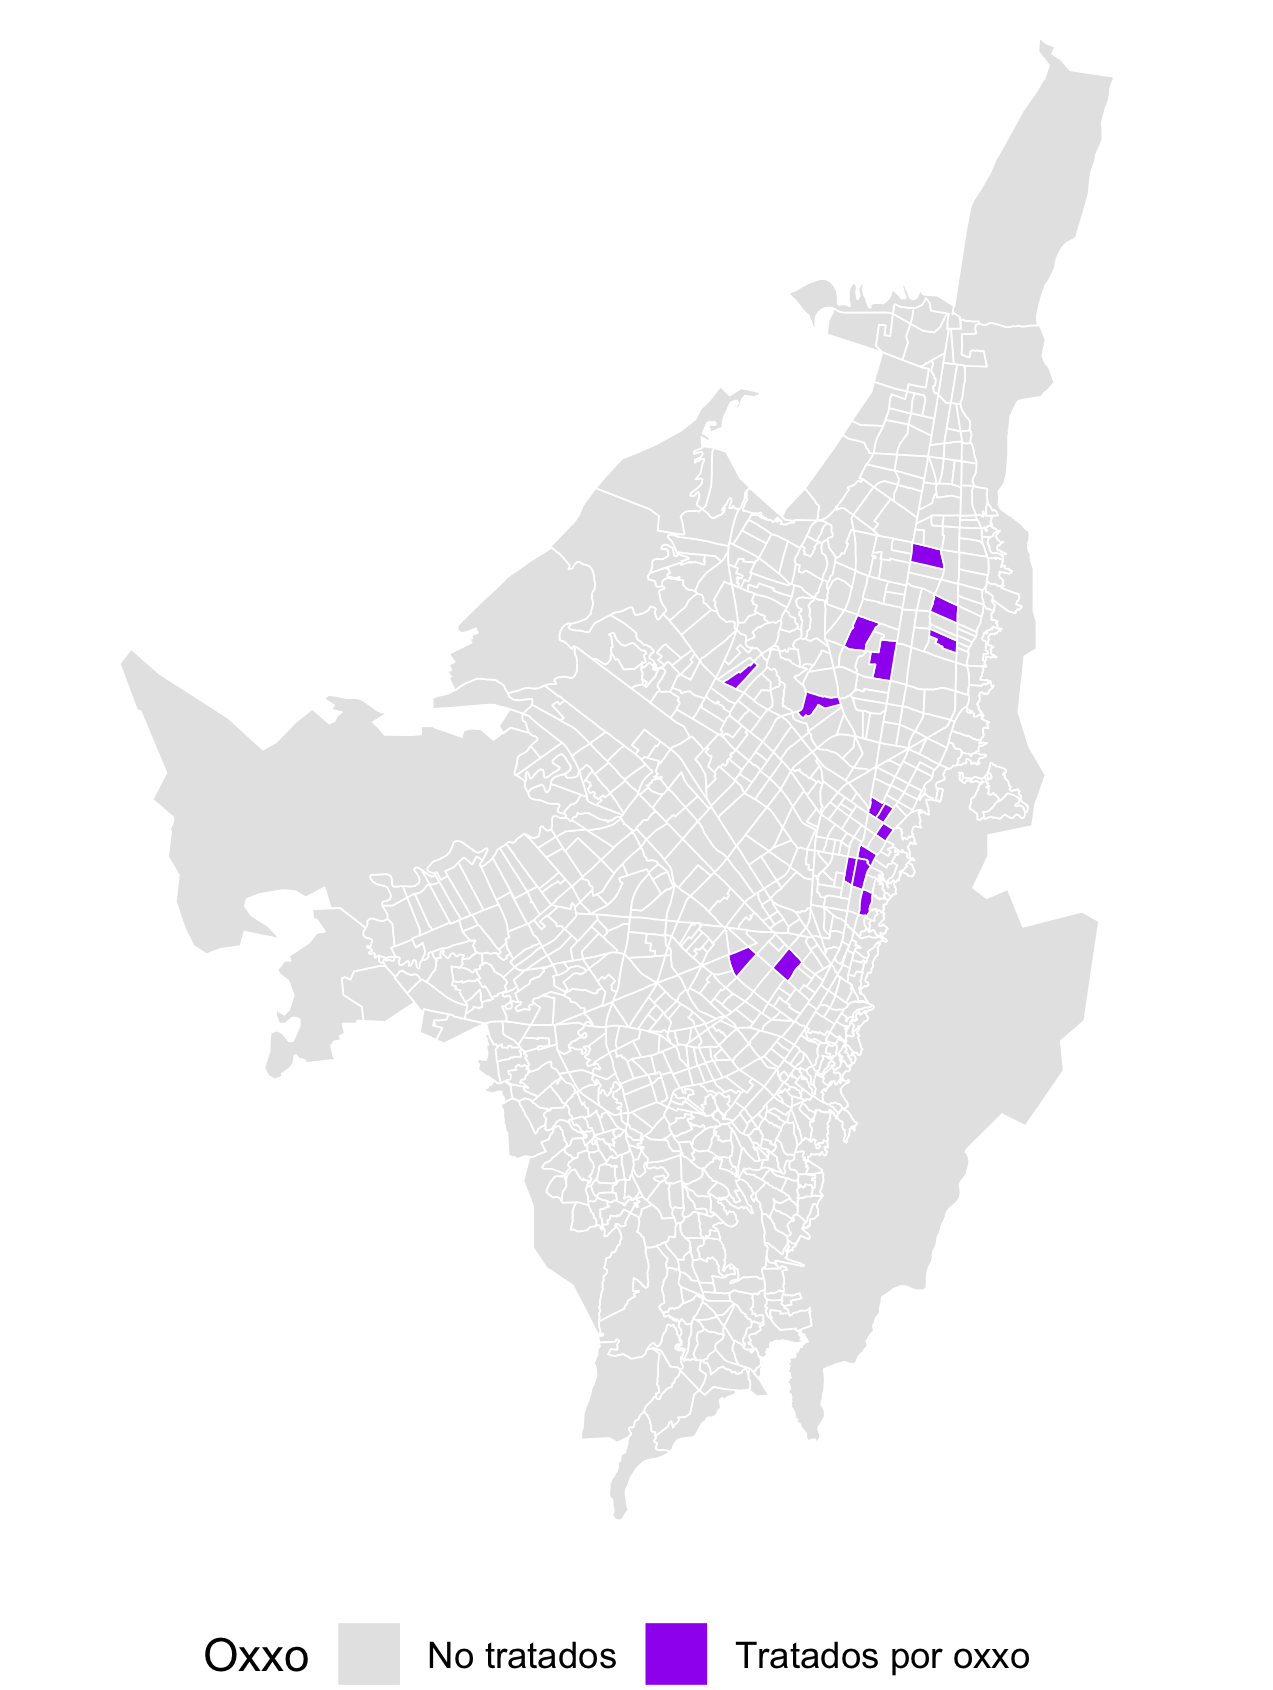
\includegraphics[width=\linewidth]{figs_oxxo_maps/mapa_oxxos_binary_2011.png}
        \caption{Panel A: OXXOs por ZAT en el 2011}
        \label{fig:panelA}
    \end{subfigure}
    \hfill
    % Top-right
    \begin{subfigure}[b]{0.4\textwidth} % Valor ajustado aquí
        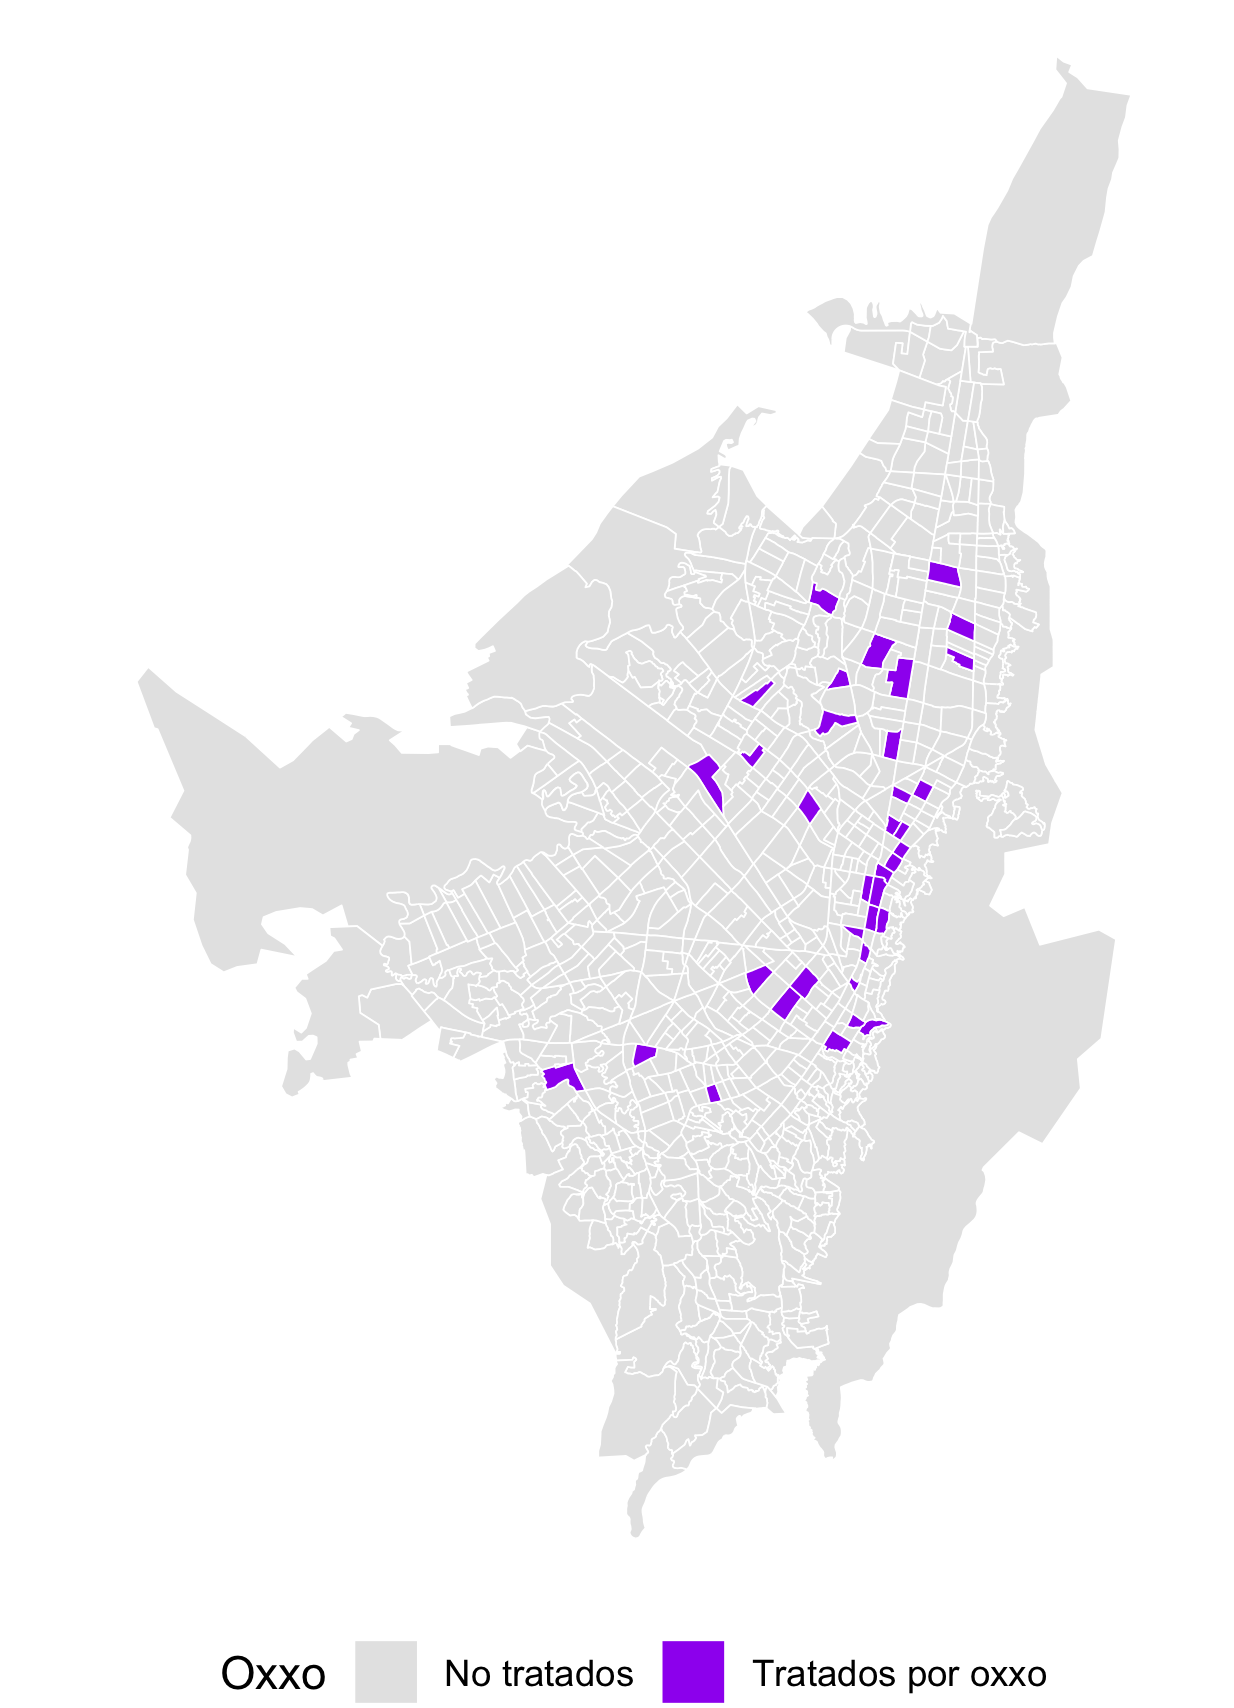
\includegraphics[width=\linewidth]{figs_oxxo_maps/mapa_oxxos_binary_2015.png}
        \caption{Panel B: OXXOs por ZAT en el 2015}
        \label{fig:panelB}
    \end{subfigure}
    
    \vspace{0.5cm}
    
    % Bottom-left
    \begin{subfigure}[b]{0.4\textwidth} % Valor ajustado aquí
        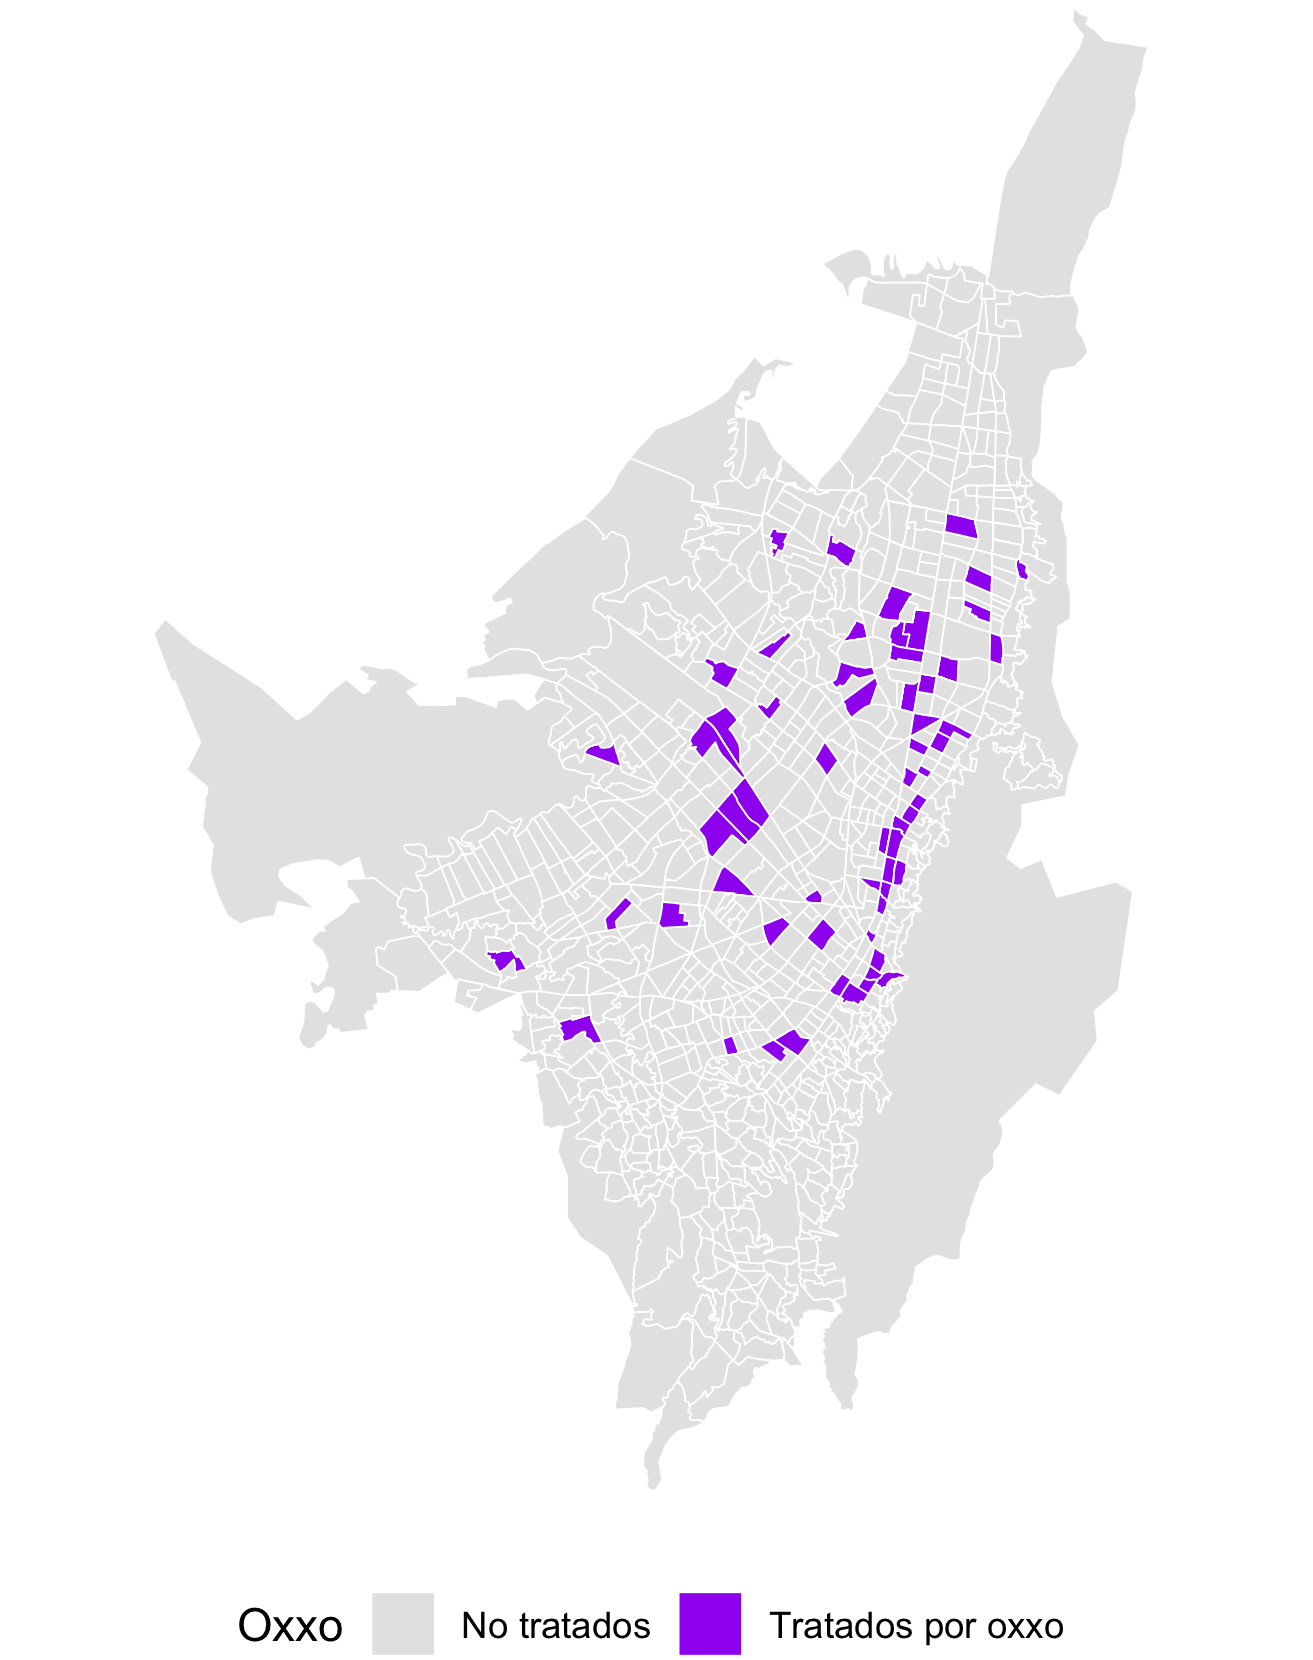
\includegraphics[width=\linewidth]{figs_oxxo_maps/mapa_oxxos_binary_2019.png}
        \caption{Panel C: OXXOs por ZAT en el 2019}
        \label{fig:panelC}
    \end{subfigure}
    \hfill
    % Bottom-right
    \begin{subfigure}[b]{0.4\textwidth} % Valor ajustado aquí
        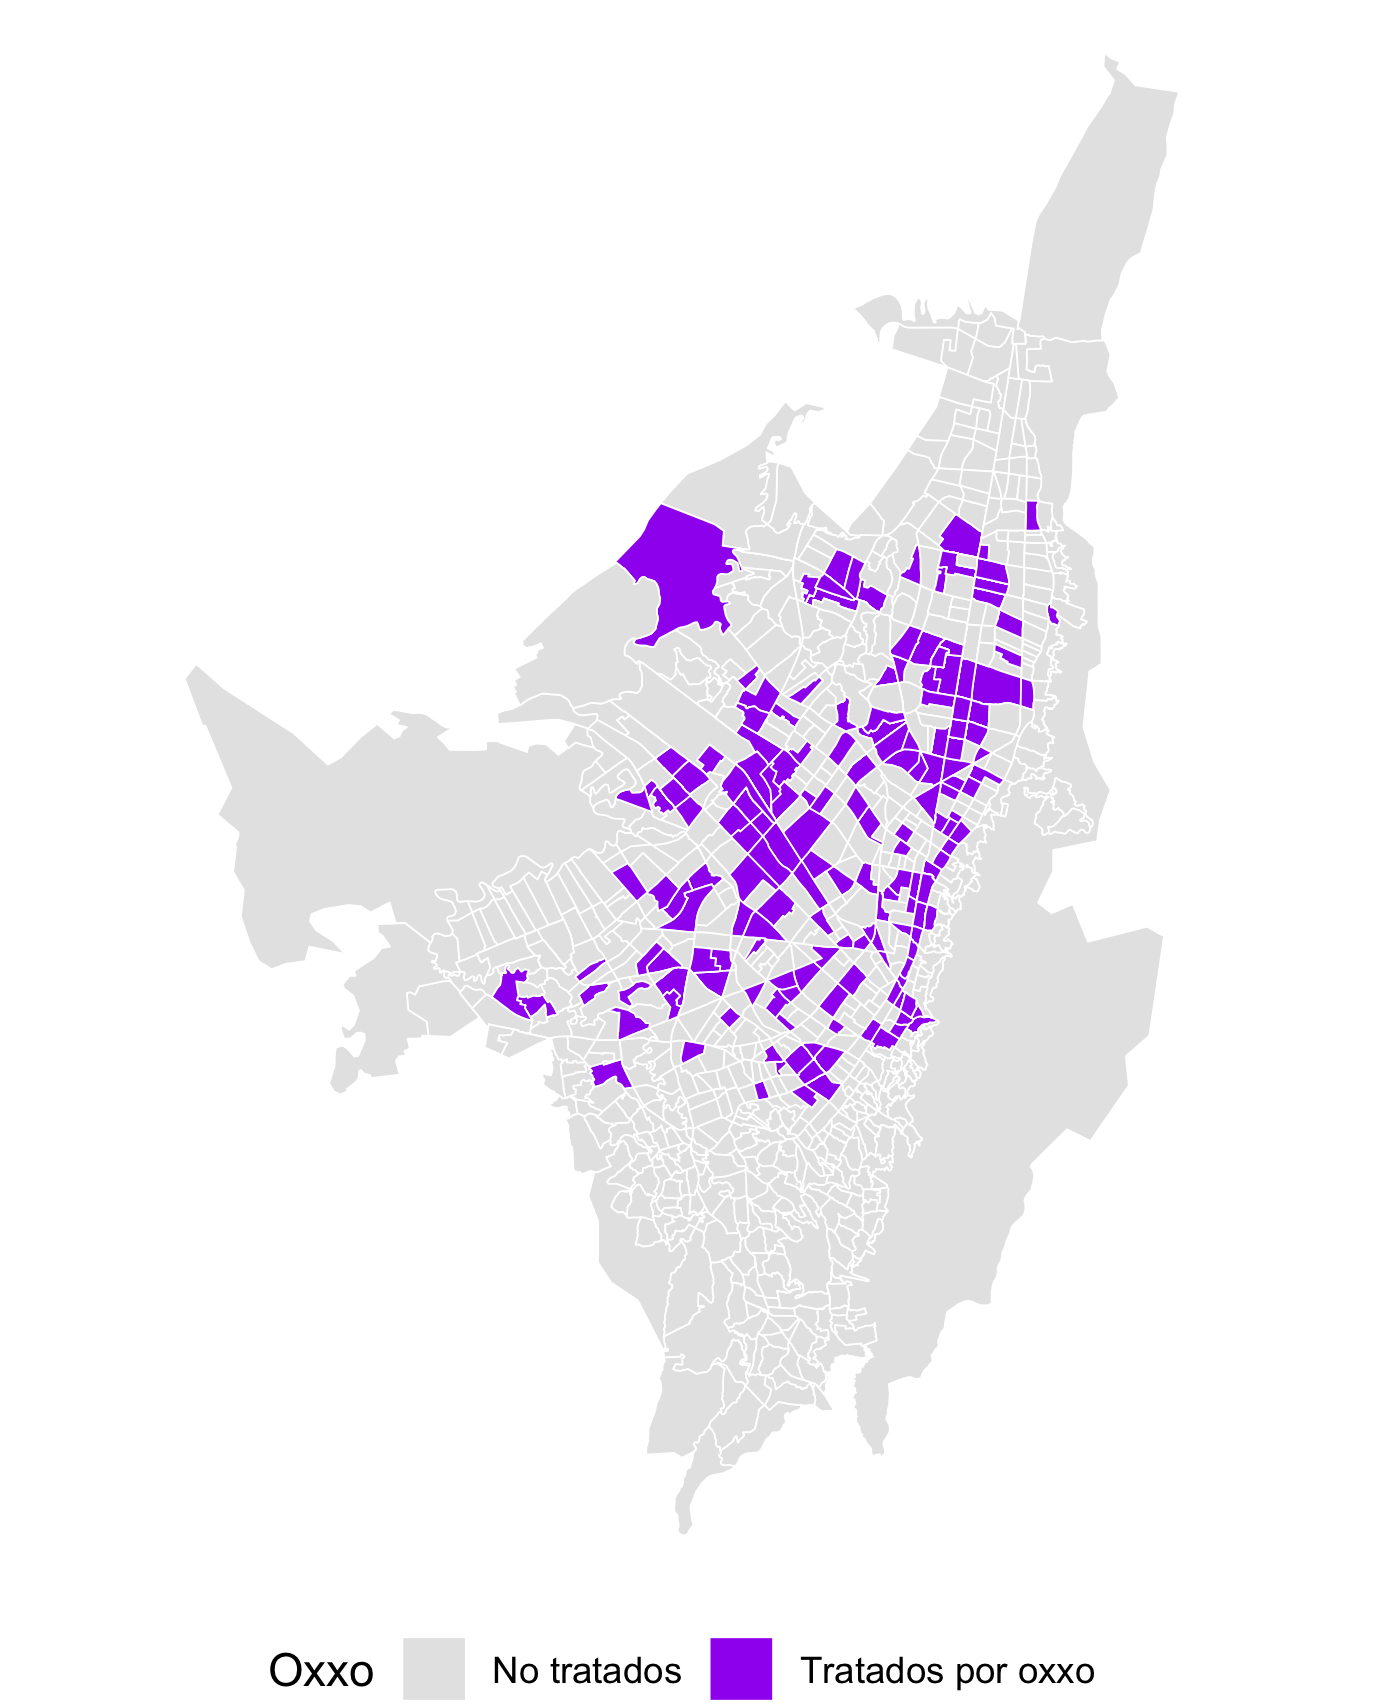
\includegraphics[width=\linewidth]{figs_oxxo_maps/mapa_oxxos_binary_2023.png}
        \caption{Panel D: OXXOs por ZAT en el 2023}
        \label{fig:panelD}
    \end{subfigure}
    
    \caption{
        \textbf{Evolución de la presencia de OXXOs por ZAT}
    }
    \label{fig:fourpanel}
\end{figure}


\begin{table} [H]
  \centering
  \caption{Proporción de Independientes y ZATs a lo largo del tiempo}
  \label{tab:independientes_zats}
  \begin{adjustbox}{width=\textwidth,center} % Add this environment
    \begin{tabular}{lcccccccc}
      \toprule
      & \multicolumn{4}{c}{\textbf{Tratados}} & \multicolumn{4}{c}{\textbf{Aún sin tratar}} \\
      \cmidrule(lr){2-5} \cmidrule(lr){6-9}
      & \textbf{2011} & \textbf{2015} & \textbf{2019} & \textbf{2023} & \textbf{2011} & \textbf{2015} & \textbf{2019} & \textbf{2023} \\
      \midrule
      proporción independientes & 0.335 & 0.284 & 0.199 & 0.302 & 0.277 & 0.260 & 0.207 & 0.301 \\
      & (0.042) & (0.017) & (0.014) & (0.011) & (0.009) & (0.008) & (0.008) & (0.009) \\
      \midrule
      ZATs & 16 & 36 & 61 & 171 & 880 & 860 & 835 & 725 \\
      \bottomrule
    \end{tabular}
  \end{adjustbox} % End the adjustbox environment
  \parbox[t]{\textwidth}{%
    \vspace{0.5em}
    \small \textit{Nota:} El valor entre paréntesis indica la desviación estándar. Esta tabla muestra la proporción de individuos "independientes" y el número total de ZATs (zonas de asentamiento temporal) para las zonas tratadas y no tratadas a lo largo de los años.
  }
\end{table}

\begin{table} [H]
  \centering
  \caption{Proporción de Independientes a lo largo del tiempo}
  \label{tab:proporcion_independientes}
  \begin{tabular}{l *{4}{p{1.5cm}}} % Use p{...} to set fixed column widths
    \toprule
    & \textbf{2011} & \textbf{2015} & \textbf{2019} & \textbf{2023} \\
    \midrule
    \textbf{proporción independientes} & 0.058 & 0.024 & -0.008 & 0.001 \\
    \bottomrule
  \end{tabular}
  \parbox[t]{\textwidth}{%
    \vspace{0.5em}
    \small \textit{Nota:} Esta tabla muestra la proporción de individuos "independientes" a lo largo de los años.
  }
\end{table}


\section{Variables de control}

\begin{table} [H]
  \centering
  \caption{Diferencias de medias entre tratados y nunca tratados}
  \label{tab:diferencias_medias}
  \begin{adjustbox}{width=\textwidth,center}
    \begin{tabular}{l c c c}
      \toprule
      \multicolumn{1}{c}{} & \multicolumn{1}{c}{\textbf{Nunca tratados}} & \multicolumn{1}{c}{\textbf{Tratados}} & \multicolumn{1}{c}{\textbf{diferencia de medias}} \\
      \midrule
       \midrule
      \multicolumn{4}{l}{\textbf{Línea base}} \\
      \midrule
      densidad urbana por upz 2009 & $2.81e+11$ & $2.85e+11$ & $3.94e+09$ \\
      & $(8.16e+09)$ & $(1.91e+10)$ & \\
      área urbana por upz 2009 & $3.90e+11$ & $3.62e+11$ & $-2.79e+10$ \\
      & $(7.62e+09)$ & $(1.37e+10)$ & \\
      poblacion urbana por upz 2009 & 78937.337 & 68880.655 & $-1.01e+04^{**}$ \\
      & $(2177.024)$ & $(4302.714)$ & \\
      Habitantes por localidad en 2007 & 481.997 & 473.073 & -8.924 \\
      & (11.180) & (26.920) & \\
      cantidad de personas por hogar 2007 & 3.522 & 3.298 & $-0.225^{***}$ \\
      & (0.015) & (0.030) & \\
      Indice de condiciones de vida 2007 & 89.121 & 91.724 & $2.603^{***}$ \\
      & (0.151) & (0.216) & \\
      gasto promedio mensual 2007 & $1.02e+06$ & $1.28e+06$ & $2.54e+05^{***}$ \\
      & $(22613.352)$ & $(50141.458)$ & \\
      \midrule
      \multicolumn{4}{l}{\textbf{Controles fijos}} \\
      \midrule
      estrato promedio & 2.722 & 3.483 & $0.761^{***}$ \\
      & (0.047) & (0.073) & \\
      Estaciones de transmilenio cercanas & 1.746 & 3.433 & $1.687^{***}$ \\
      & (0.088) & (0.221) & \\
      tiene acceso al transmilenio & 0.491 & 0.795 & $0.304^{***}$ \\
      & (0.019) & (0.031) & \\
      Cantidad acceso a vías arteriales & 3.830 & 6.234 & $2.404^{***}$ \\
      & (0.103) & (0.292) & \\
      Tiene acceso a vías arteriales & 0.913 & 1.000 & $0.087^{***}$ \\
      & (0.010) & (0.000) & \\
      \midrule
      \midrule
      ZATs & 725 & 171 & 896 \\
      \bottomrule
    \end{tabular}
  \end{adjustbox}
\end{table}

Identifiquen e incluyan variables de control pertinentes que puedan afectar la variable dependiente de su estudio. Para cada variable de control:
Justificación: Proporcionen un argumento sólido respaldado por la literatura existente o datos empíricos que justifique su inclusión.
Análisis Descriptivo: Analicen el impacto de estas variables con estadísticas descriptivas para los dos grupos de análisis.

Análisis del Impacto de las Variables de Control
Analicen cómo estas variables de control afectan sus resultados. Discutan si actúan
efectivamente como buenos controles en su modelo de investigación. Mencionen
brevemente cualquier problema que se presente, como posibles sesgos o limitaciones en los
datos. (Máximo 200 palabras)


\section{Referencias}

\printbibliography

PARA OBTENER SHAPEFILES ZATs: \url{https://datosabiertos-transmilenio.hub.arcgis.com/datasets/e6cf3d5c3ec2499e8a959fa3aee8fbd4_0/explore?location=4.678900%2C-74.085690%2C13.18}


\appendix
\counterwithin{table}{section}
\counterwithin{figure}{section}

\section{Controles línea base por cohortes}

\begin{table} [H]
  \centering
  \caption{2011 - entre tratados y nunca tratados}
  \label{tab:comparacion_2011}
  \begin{tabular}{l c c c}
    \toprule
    & \textbf{Aún sin tratar} & \textbf{Tratados} & \textbf{diferencia de medias} \\
    \midrule
    \multicolumn{4}{l}{\textbf{Línea base}} \\
    \midrule
    poblacion urbana por upz 2009 & 77473.727 & 51955.062 & $-2.55e+04^{*}$ \\
    & (1971.452) & (9851.411) & \\
    densidad urbana por upz 2009 & $2.82e+11$ & $2.98e+11$ & $1.60e+10$ \\
    & $(7.58e+09)$ & $(6.79e+10)$ & \\
    área urbana por upz 2009 & $3.85e+11$ & $3.69e+11$ & $-1.63e+10$ \\
    & $(6.76e+09)$ & $(5.57e+10)$ & \\
    Habitantes por localidad en 2007 & 481.890 & 392.478 & -89.413 \\
    & (10.465) & (87.608) & \\
    cantidad de personas por hogar 2007 & 3.489 & 2.971 & $-0.518^{***}$ \\
    & (0.014) & (0.116) & \\
    Indice de condiciones de vida 2007 & 89.539 & 93.955 & $4.416^{***}$ \\
    & (0.134) & (0.640) & \\
    gasto promedio mensual 2007 & $1.06e+06$ & $1.79e+06$ & $7.35e+05^{***}$ \\
    & (20917.105) & (1.21e+05) & \\
    \midrule
    \multicolumn{4}{l}{\textbf{Controles fijos}} \\
    \midrule
    estrato promedio & 2.864 & 3.801 & $0.937^{***}$ \\
    & (0.042) & (0.193) & \\
    Estaciones de transmilenio cercanas & 2.039 & 3.688 & $1.649^{**}$ \\
    & (0.087) & (0.454) & \\
    tiene acceso al transmilenio & 0.543 & 0.875 & $0.332^{**}$ \\
    & (0.017) & (0.085) & \\
    Cantidad acceso a vías arteriales & 4.223 & 7.938 & $3.715^{***}$ \\
    & (0.103) & (0.292) & \\
    Tiene acceso a vías arteriales & 0.928 & 1.000 & 0.072 \\
    & (0.009) & (0.000) & \\

    \midrule
    \textbf{ZATs} & 880 & 16 & 896 \\
    \bottomrule
  \end{tabular}
\end{table}

\begin{table} [H]
  \centering
  \caption{2015 - entre tratados y nunca tratados}
  \label{tab:comparacion_2015}
  \begin{tabular}{l c c c}
    \toprule
    & \textbf{Aún sin tratar} & \textbf{Tratados} & \textbf{diferencia de medias} \\
    \midrule
    \multicolumn{4}{l}{\textbf{Línea base}} \\
    \midrule
    poblacion urbana por upz 2009 & 77975.227 & 54151.833 & $-2.38e+04^{**}$ \\
    densidad urbana por upz 2009 & $2.81e+11$ & $3.10e+11$ & $2.96e+10$ \\
    & $(7.63e+09)$ & $(4.47e+10)$ & \\
    área urbana por upz 2009 & $3.86e+11$ & $3.58e+11$ & $-2.82e+10$ \\
    & $(6.83e+09)$ & $(3.53e+10)$ & \\
    & (1997.734) & (7560.578) & \\
    Habitantes por localidad en 2007 & 484.916 & 369.880 & -115.035$^{**}$ \\
    & (10.529) & (58.628) & \\
    cantidad de personas por hogar 2007 & 3.497 & 3.075 & $-0.422^{***}$ \\
    & (0.014) & (0.079) & \\
    Indice de condiciones de vida 2007 & 89.501 & 92.409 & $2.908^{***}$ \\
    & (0.136) & (0.591) & \\
    gasto promedio mensual 2007 & $1.06e+06$ & $1.47e+06$ & $4.15e+05^{***}$ \\
    & (21062.412) & (1.15e+05) & \\
    \midrule
    \multicolumn{4}{l}{\textbf{Controles fijos}} \\
    \midrule
    estrato promedio & 2.842 & 3.735 & $0.893^{***}$ \\
    & (0.042) & (0.161) & \\
    Estaciones de transmilenio cercanas & 1.984 & 4.083 & $2.100^{**}$ \\
    & (0.087) & (0.422) & \\
    tiene acceso al transmilenio & 0.535 & 0.889 & $0.354^{**}$ \\
    & (0.017) & (0.053) & \\
    Cantidad acceso a vías arteriales & 4.176 & 7.000 & $2.824^{***}$ \\
    & (0.103) & (0.715) & \\
    Tiene acceso a vías arteriales & 0.927 & 1.000 & $0.073^{*}$ \\
    & (0.009) & (0.000) & \\
    \midrule
    \textbf{ZATs} & 860 & 36 & 896 \\
    \bottomrule
  \end{tabular}
\end{table}

\begin{table} [H]
  \centering
  \caption{2019 - entre tratados y nunca tratados}
  \label{tab:comparacion_2019}
  \begin{tabular}{l c c c}
    \toprule
    & \textbf{Aún sin tratar} & \textbf{Tratados} & \textbf{diferencia de medias} \\
    \midrule
    \multicolumn{4}{l}{\textbf{Línea base}} \\
    \midrule
    poblacion urbana por upz 2009 & 78594.207 & 55442.590 & $-2.32e+04^{**}$ \\
    densidad urbana por upz 2009 & $2.79e+11$ & $3.17e+11$ & $3.79e+10$ \\
    & $(7.70e+09)$ & $(3.37e+10)$ & \\
    área urbana por upz 2009 & $3.88e+11$ & $3.43e+11$ & $-4.48e+10$ \\
    & $(6.94e+09)$ & $(2.54e+10)$ & \\
    & (2015.555) & (7020.198) & \\
    Habitantes por localidad en 2007 & 485.354 & 411.027 & -74.327$^{*}$ \\
    & (10.662) & (44.380) & \\
    cantidad de personas por hogar 2007 & 3.503 & 3.153 & $-0.350^{***}$ \\
    & (0.014) & (0.059) & \\
    Indice de condiciones de vida 2007 & 89.440 & 92.409 & $2.615^{***}$ \\
    & (0.138) & (0.424) & \\
    gasto promedio mensual 2007 & $1.05e+06$ & $1.41e+06$ & $3.60e+05^{***}$ \\
    & (21241.687) & (88739.694) & \\
    \midrule
    \multicolumn{4}{l}{\textbf{Controles fijos}} \\
    \midrule
    estrato promedio & 2.818 & 3.671 & $0.853^{***}$ \\
    & (0.043) & (0.141) & \\
    Estaciones de transmilenio cercanas & 1.941 & 3.803 & $1.862^{**}$ \\
    & (0.087) & (0.352) & \\
    tiene acceso al transmilenio & 0.528 & 0.836 & $0.308^{***}$ \\
    & (0.017) & (0.048) & \\
    Cantidad acceso a vías arteriales & 4.111 & 6.721 & $2.610^{***}$ \\
    & (0.102) & (0.550) & \\
    Tiene acceso a vías arteriales & 0.925 & 1.000 & $0.075^{**}$ \\
    & (0.009) & (0.000) & \\
    \midrule
    \textbf{ZATs} & 896 & 61 & 896 \\
    \bottomrule
  \end{tabular}
\end{table}

\begin{table} [H]
  \centering
  \caption{2023 - entre tratados y nunca tratados}
  \label{tab:comparacion_tratamientos}
  \begin{tabular}{l c c c}
    \toprule
    & \textbf{Aún sin tratar} & \textbf{Tratados} & \textbf{diferencia de medias} \\
    \midrule
    \multicolumn{4}{l}{\textbf{Línea base}} \\
    \midrule
    poblacion urbana por upz 2009 & 78937.337 & 68880.655 & $-1.01e+04^{**}$ \\
    densidad urbana por upz 2009 & $2.81e+11$ & $2.85e+11$ & $3.94e+09$ \\
    & $(8.16e+09)$ & $(1.91e+10)$ & \\
    área urbana por upz 2009 & $3.90e+11$ & $3.62e+11$ & $-2.79e+10$ \\
    & $(7.62e+09)$ & $(1.37e+10)$ & \\
    & (2177.024) & (4302.714) & \\
    Habitantes por localidad en 2007 & 481.997 & 473.073 & -8.924 \\
    & (11.180) & (26.920) & \\
    cantidad de personas por hogar 2007 & 3.522 & 3.298 & $-0.225^{***}$ \\
    & (0.015) & (0.030) & \\
    Indice de condiciones de vida 2007 & 89.121 & 91.724 & $2.603^{***}$ \\
    & (0.151) & (0.216) & \\
    gasto promedio mensual 2007 & $1.02e+06$ & $1.28e+06$ & $2.54e+05^{***}$ \\
    & (22613.352) & (50141.458) & \\
    \midrule
    \multicolumn{4}{l}{\textbf{Controles fijos}} \\
    \midrule
        estrato promedio & 2.722 & 3.483 & $0.761^{***}$ \\
    & (0.047) & (0.073) & \\
     Estaciones de transmilenio cercanas & 1.746 & 3.433 & $1.687^{***}$ \\
    & (0.088) & (0.221) & \\
    tiene acceso al transmilenio & 0.491 & 0.795 & $0.304^{***}$ \\
    & (0.019) & (0.031) & \\
    Cantidad acceso a vías arteriales & 3.830 & 6.234 & $2.404^{***}$ \\
    & (0.103) & (0.292) & \\
    Tiene acceso a vías arteriales & 0.913 & 1.000 & $0.087^{***}$ \\
    & (0.010) & (0.000) & \\
    \midrule
    \midrule
    \textbf{ZATs} & 725 & 171 & 896 \\
    \bottomrule
  \end{tabular}
\end{table}

\section{Controles rezagados de cadenas de descuento}

\begin{table} [H]
  \centering
  \caption{Tabla de Resultados 2015}
  \label{tab:d1}
  \begin{tabular}{l c c c}
    \toprule
    & \textbf{Aún sin tratar} & \textbf{Tratados} & \textbf{diferencia de medias} \\
    \midrule
    Tiene D1 & 0.050 & 0.222 & $0.172^{***}$ \\
    & (0.007) & (0.070) & \\
    \midrule
    Cantidad de D1s & 0.062 & 0.278 & $0.216^{***}$ \\
    & (0.010) & (0.094) & \\
    \midrule
    ZATs & 860 & 36 & 896 \\
    \bottomrule
  \end{tabular}
\end{table}

\begin{table} [H]
  \centering
  \caption{Tabla de Resultados 2019}
  \label{tab:d1_jb_ara}
  \begin{tabular}{l c c c}
    \toprule
    & \textbf{Aún sin tratar} & \textbf{Tratados} & \textbf{diferencia de medias} \\
    \midrule
    Tiene J\&B & 0.083 & 0.098 & 0.016 \\
    & (0.010) & (0.038) & \\
    Tiene D1 & 0.170 & 0.410 & $0.240^{***}$ \\
    & (0.013) & (0.063) & \\
    Tiene ARA & 0.081 & 0.148 & $0.066^{*}$ \\
    & (0.009) & (0.046) & \\
    Cantidad de J\&B & 0.168 & 0.230 & 0.062 \\
    & (0.033) & (0.120) & \\
    Cantidad de D1s & 0.229 & 0.557 & $0.329^{***}$ \\
    & (0.022) & (0.098) & \\
    Cantidad de ARAs & 0.103 & 0.197 & $0.094^{*}$ \\
    & (0.013) & (0.069) & \\
    \midrule
    ZATs & 835 & 61 & 896 \\
    \bottomrule
  \end{tabular}
\end{table}

\begin{table} [H]
  \centering
  \caption{2023 - entre tratados y nunca tratados}
  \label{tab:d1_ara_2023}
  \begin{tabular}{l c c c}
    \toprule
    & \textbf{Aún sin tratar} & \textbf{Tratados} & \textbf{diferencia de medias} \\
    \midrule
    Tiene D1 & 0.214 & 0.456 & $0.242^{***}$ \\
    & (0.015) & (0.038) & \\
    Tiene ARA & 0.109 & 0.246 & $0.137^{***}$ \\
    & (0.012) & (0.033) & \\
    Cantidad de D1s & 0.288 & 0.865 & $0.577^{***}$ \\
    & (0.025) & (0.118) & \\
    Cantidad de ARAs & 0.143 & 0.357 & $0.213^{***}$ \\
    & (0.017) & (0.056) & \\
    \midrule
    ZATs & 725 & 171 & 896 \\
    \bottomrule
  \end{tabular}
\end{table}


\section{Controles por diferencias entre cortes transversales}
\begin{figure}[p] % Allow placement on a separate page
    \centering
    % Top-left
    \begin{subfigure}[b]{0.4\textwidth}
        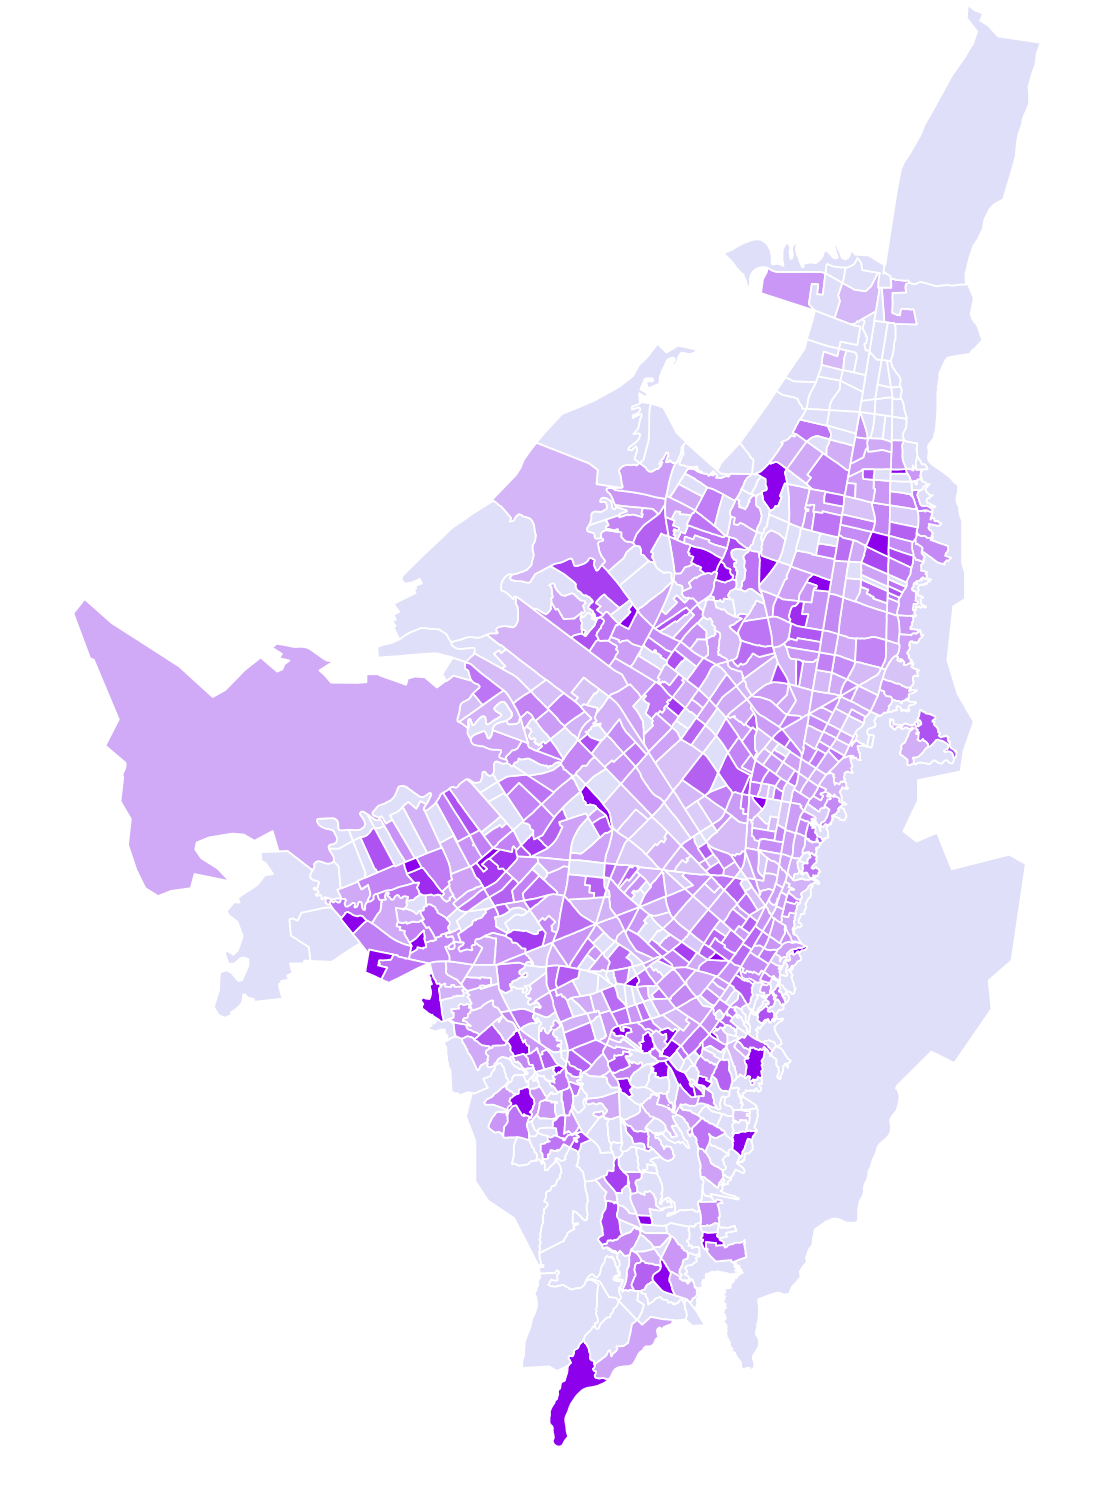
\includegraphics[width=\linewidth]{figs_dep_maps/mapa_dep_2011.png}
        \caption{Panel A: Two-EV Mixture Fit}
        \label{fig:panelA}
    \end{subfigure}
    \hfill
    % Top-right
    \begin{subfigure}[b]{0.4\textwidth}
        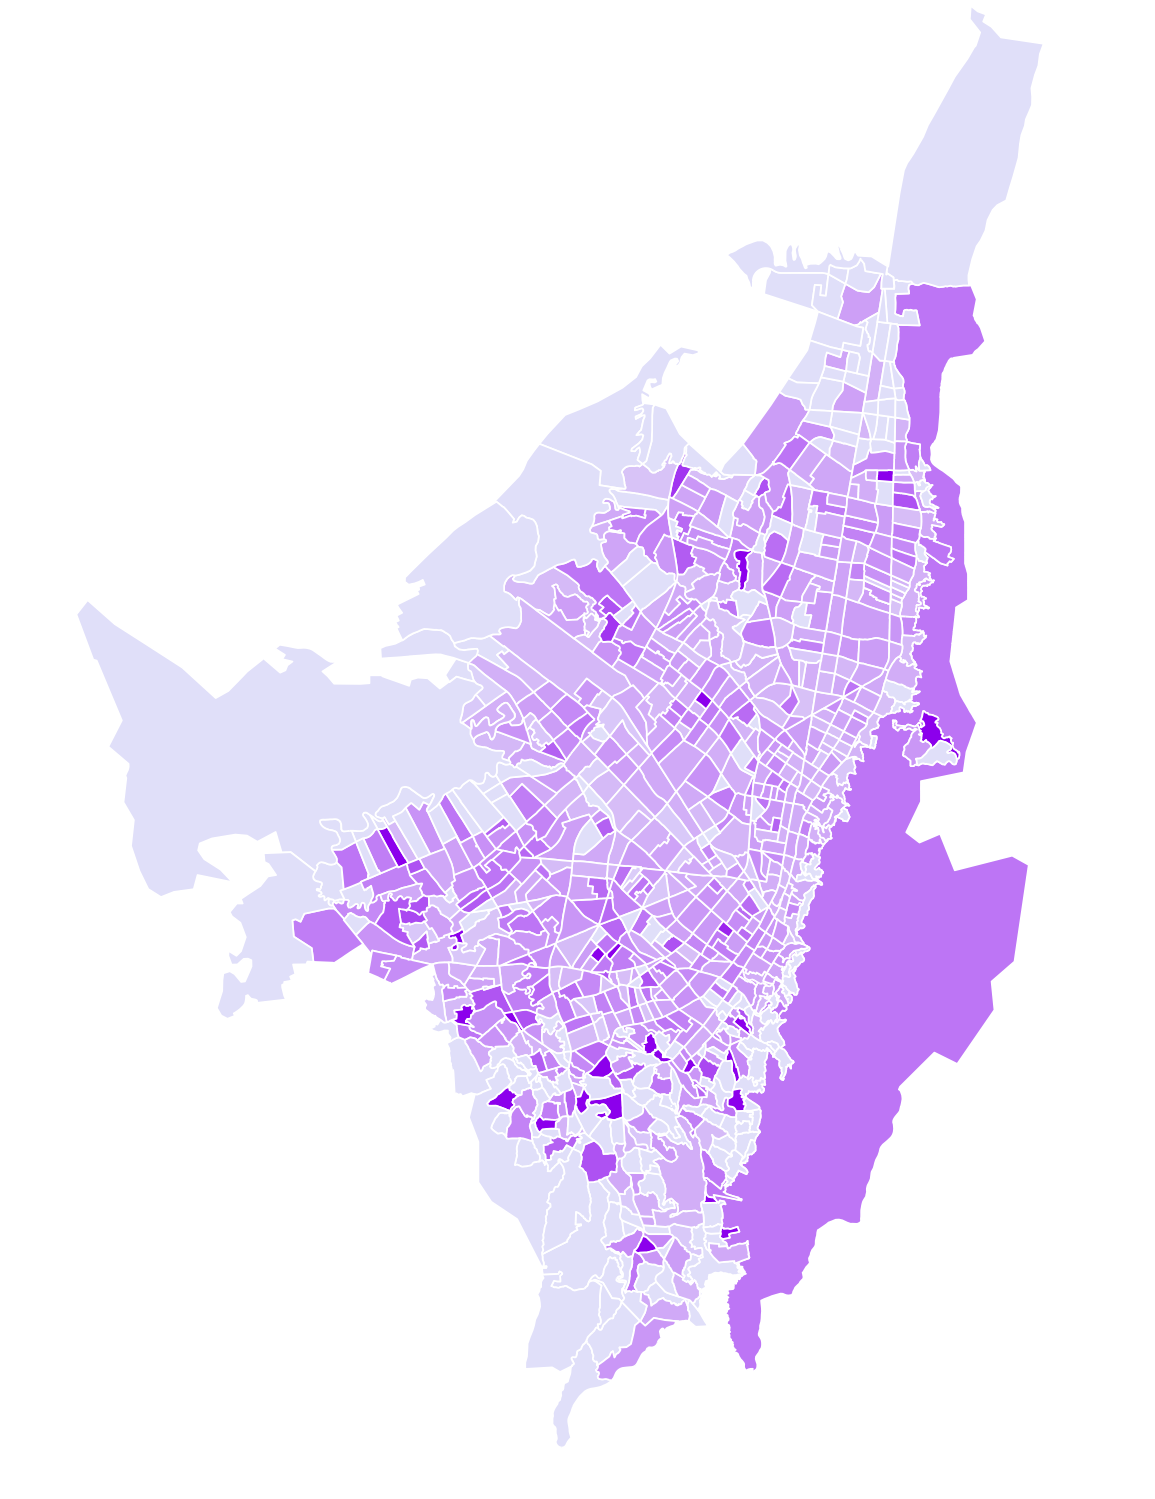
\includegraphics[width=\linewidth]{figs_dep_maps/mapa_dep_2015.png}
        \caption{Panel B: Two-Normal Mixture Fit}
        \label{fig:panelB}
    \end{subfigure}
    
    \vspace{0.5cm}
    
    % Bottom-left
    \begin{subfigure}[b]{0.4\textwidth}
        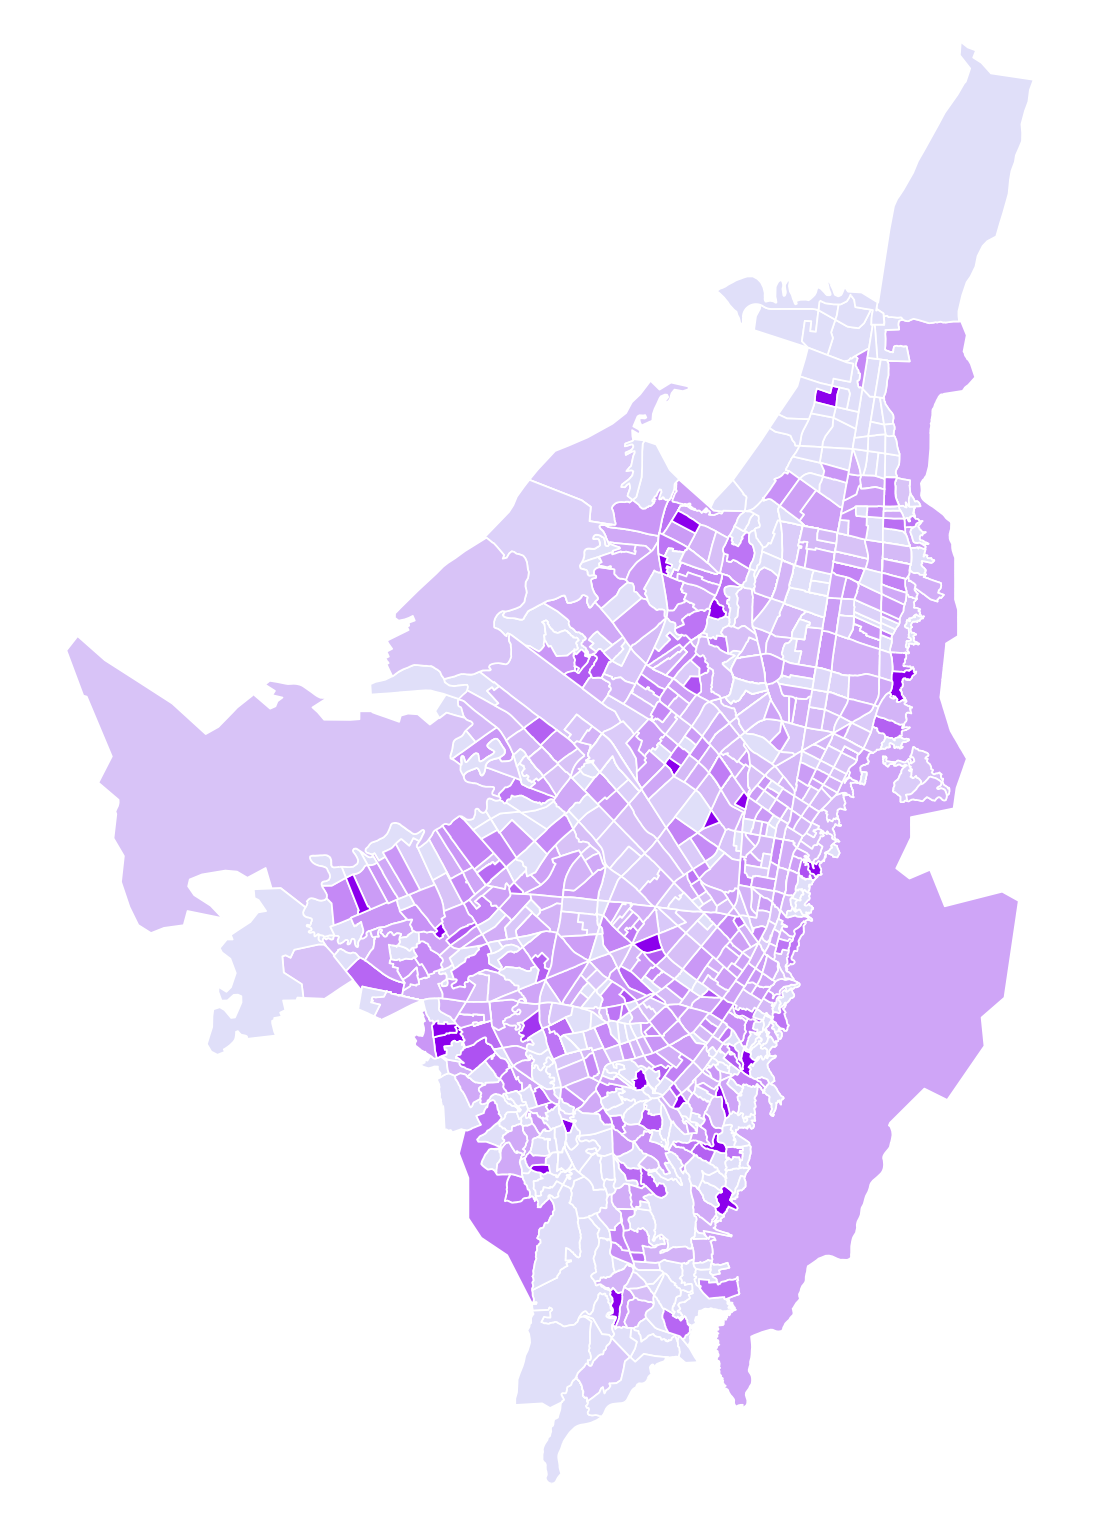
\includegraphics[width=\linewidth]{figs_dep_maps/mapa_dep_2019.png}
        \caption{Panel C: Three-EV Mixture Fit}
        \label{fig:panelC}
    \end{subfigure}
    \hfill
    % Bottom-right
    \begin{subfigure}[b]{0.4\textwidth}
        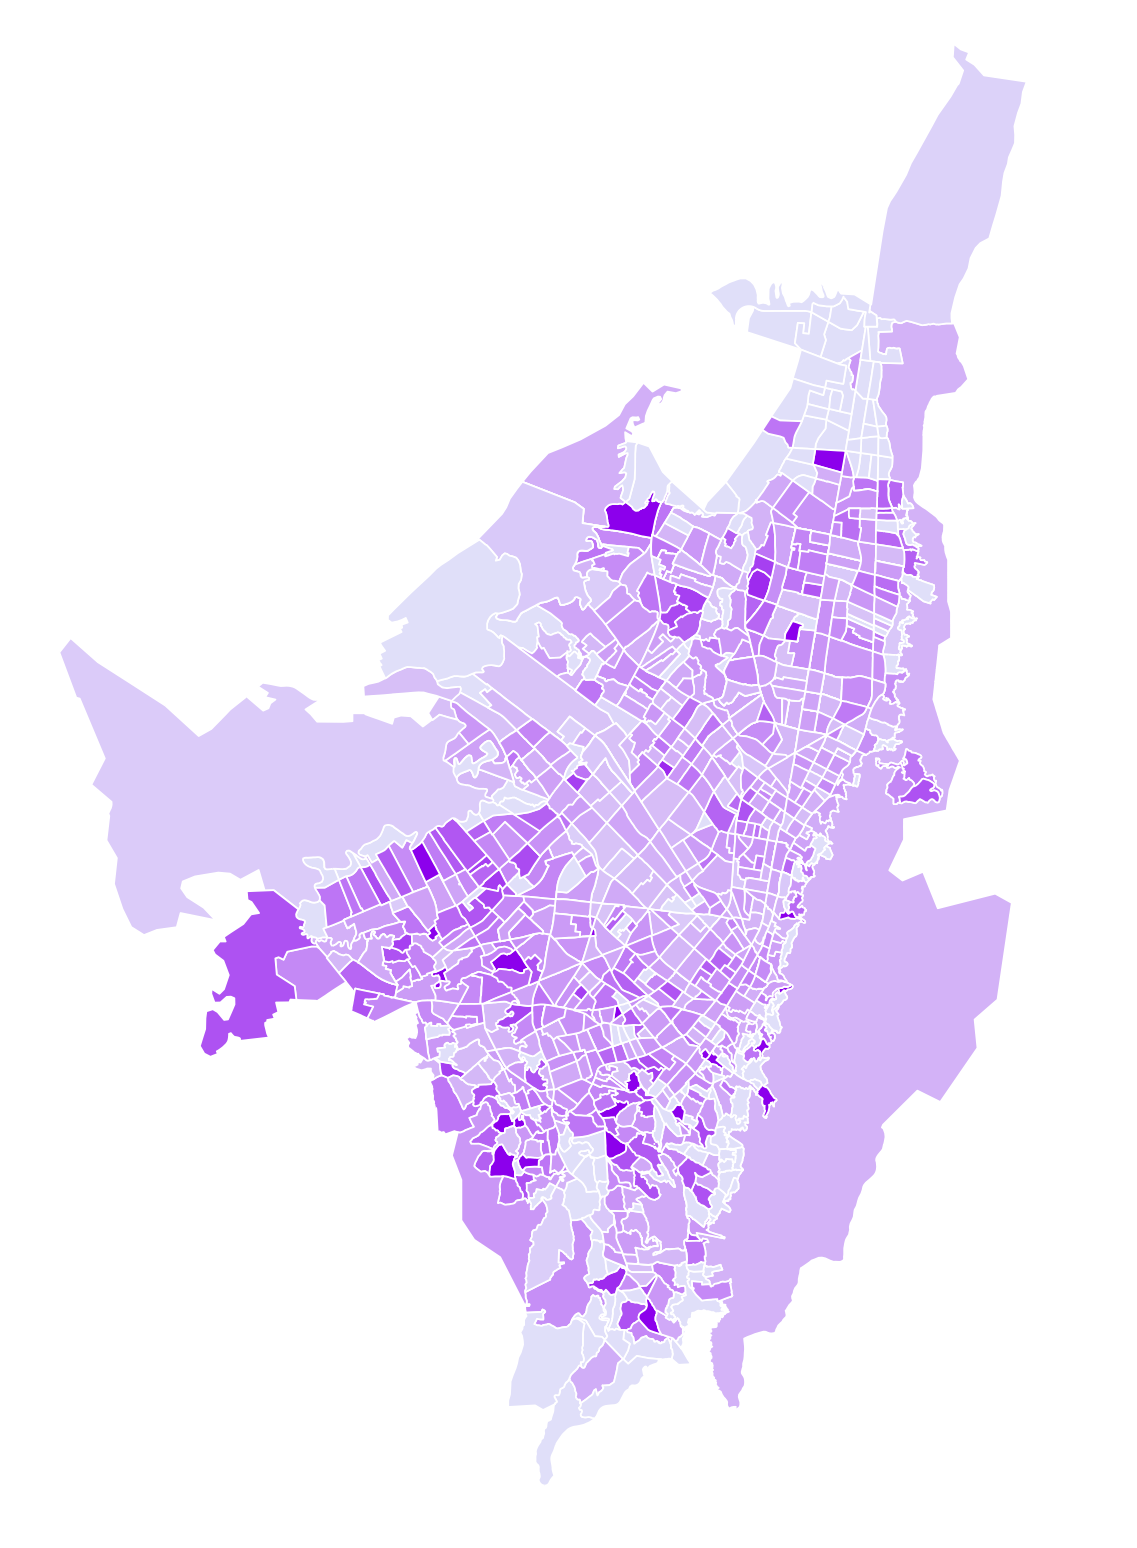
\includegraphics[width=\linewidth]{figs_dep_maps/mapa_dep_2023.png}
        \caption{Panel D: Three-Normal Mixture Fit}
        \label{fig:panelD}
    \end{subfigure}
    
    % Aquí se agrega la imagen de referencia
    \vspace{0.3cm} % Espacio entre los paneles y la imagen de referencia
    \begin{minipage}{\textwidth} % Un minipage para the control total
        \begin{flushright} % Para alinear a la derecha
            
\includegraphics[width=0.7\textwidth]{figs_dep_maps/clasificacion.png} % Ajusta el ancho y el nombre
        \end{flushright}
    \end{minipage}
    
    \caption{
        \textbf{EM Algorithm Mixture Fits Under Varying Distributional Assumptions.}
        Four-panel figure comparing estimated mixture distributions obtained using the EM algorithm under different modeling assumptions. Each panel corresponds to one of the four cases: two or three components, with either Normal or Extreme Value (EV) distributions. In each panel, the fitted mixture is overlaid on the empirical distribution of the data from \texttt{Q4\_data.csv}.
    }
    \label{fig:fourpanel}
\end{figure}

\end{document}
